\documentclass{standalone}
\usepackage{tikz}
\usepackage{ctex,siunitx}
\usepackage{tkz-euclide}
\usepackage{amsmath}
\usetikzlibrary{patterns, calc}
\usetikzlibrary {decorations.pathmorphing, decorations.pathreplacing, decorations.shapes,}
\begin{document}
\small
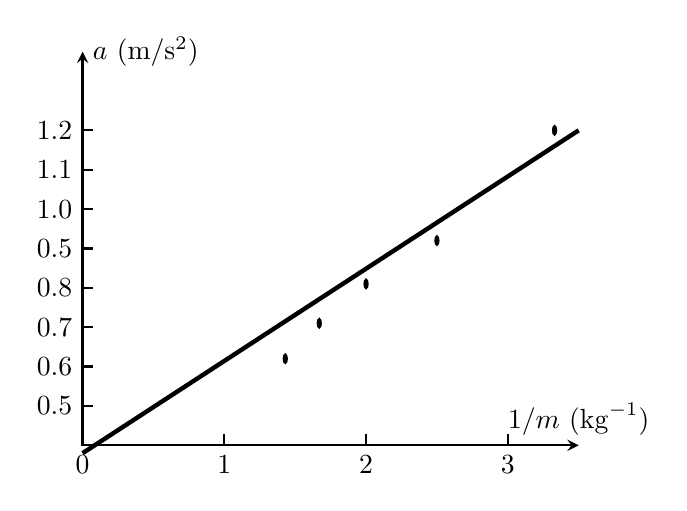
\begin{tikzpicture}[xscale=1.8,yscale=5, >=stealth, thick]
  \draw [<->](0,1.4)node [right]{$a$ (\unit{m/s^2})}--(0,.4)--(3.5,0.4)node [above]{$1/m$ (\unit{kg^{-1}})};
  \foreach \x in{0.5,0.6,...,1.2}
  {
      \draw(0,\x) --(0.07,\x);
  }
  \draw(0,1.2) --(0.07,1.2);
  \foreach \y in{1,2,3}
  {
      \draw(\y,0.4)--(\y,0.03+.4);
  }
  \draw [fill=black] (3.33  ,  1.2)  circle [radius=.3pt];
  \draw [fill=black]  (2.5  , 0.92 ) circle [radius=.3pt];
  \draw [fill=black]  (2  , .81 ) circle [radius=.3pt];
  \draw [fill=black]  (1.67  ,  .71)  circle [radius=.3pt];
  \draw [fill=black]  (1.43  ,  .62)circle [radius=.3pt];
  \draw[ultra thick](0,0.38)--(3.5,1.2);
  \node at (0,0.4)[below]{0};
  \node at (1,0.4)[below]{1};
  \node at (2,0.4)[below]{2};
  \node at (3,0.4)[below]{3};
  \node at (0,0.5)[left]{0.5};
  \node at (0,0.6)[left]{0.6};
  \node at (0,0.7)[left]{0.7};
  \node at (0,0.8)[left]{0.8};
  \node at (0,0.9)[left]{0.5};
  \node at (0,1)[left]{1.0};
  \node at (0,1.1)[left]{1.1};
  \node at (0,1.2)[left]{1.2};
\end{tikzpicture}
\end{document}